%%%%%%%%%%%%%%%%%%%%%%%%%%%%%%%%%%%%%%%%%
% FRI Data Science_report LaTeX Template
% Version 1.0 (28/1/2020)
%
% Jure Demšar (jure.demsar@fri.uni-lj.si)
%
% Based on MicromouseSymp article template by:
% Mathias Legrand (legrand.mathias@gmail.com)
% With extensive modifications by:
% Antonio Valente (antonio.luis.valente@gmail.com)
%
% License:
% CC BY-NC-SA 3.0 (http://creativecommons.org/licenses/by-nc-sa/3.0/)
%
%%%%%%%%%%%%%%%%%%%%%%%%%%%%%%%%%%%%%%%%%


%----------------------------------------------------------------------------------------
%	PACKAGES AND OTHER DOCUMENT CONFIGURATIONS
%----------------------------------------------------------------------------------------
\documentclass[fleqn,moreauthors,10pt]{ds_report}
\usepackage[english]{babel}
\usepackage{natbib}
\usepackage{float}

\graphicspath{{figures/}}



%----------------------------------------------------------------------------------------
%	ARTICLE INFORMATION
%----------------------------------------------------------------------------------------

% Header
\JournalInfo{UL FRI Data Science - Image Based Biometry}

% Type of report
\Archive{Project Report}

% Article title
\PaperTitle{Identification of amphibians using deep neural networks}

% Authors and their info
\Authors{Aljaz Mur Erzen\textsuperscript{1}}
\affiliation{\textsuperscript{1}\textit{ae4964@student.uni-lj.si, 63160011}}

% Keywords
\Keywords{Classification, Identification, Neural Network}
\newcommand{\keywordname}{Keywords}


%----------------------------------------------------------------------------------------
%	ABSTRACT
%----------------------------------------------------------------------------------------

%----------------------------------------------------------------------------------------

\begin{document}

% Makes all text pages the same height
\flushbottom

% Print the title and abstract box
\maketitle

% Removes page numbering from the first page
\thispagestyle{empty}

%----------------------------------------------------------------------------------------
%	ARTICLE CONTENTS
%----------------------------------------------------------------------------------------

\section*{Introduction}

Capture-mark-recapture (CMR) is a method commonly used in ecology to estimate an animal population's size where it is impractical to count every individual. A number of statistical models exist to estimate closed population size based on number of recaptured individuals. For most species, marking is done in a form of an attachable tag, but when it comes to amphibians (e.g. toads, newts) such tagging is impractical. Instead, some amphibian species have individual belly patterns that can be recorded and compared against on recapture.

These belly patterns are unique, at least for practical uses on small population sizes, and are somewhat time invariant, even though there are observed cases of mutating patterns. There are studies on practical uses of photo-identification for these species \cite{genecap_ampident}.

\begin{figure}[htb]\centering
	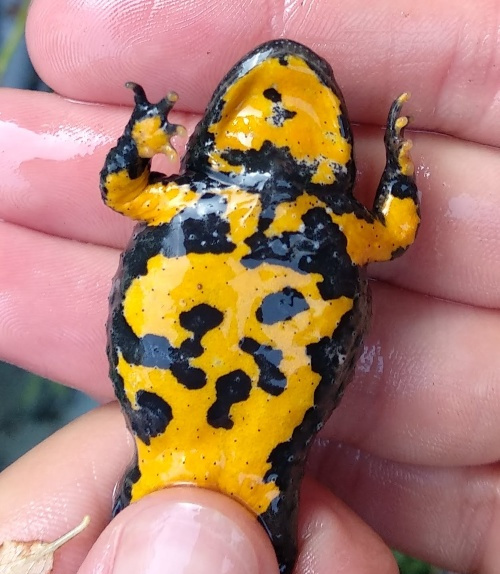
\includegraphics[width=0.49\linewidth]{hermiona_1.jpg}
	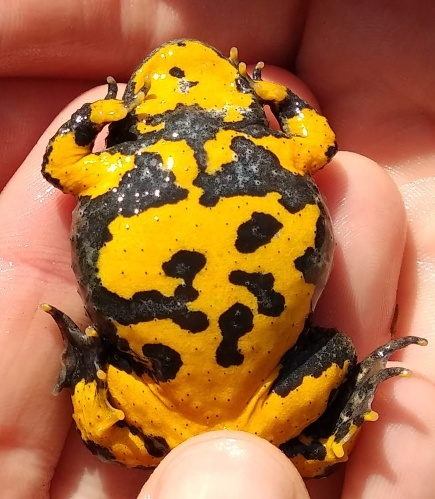
\includegraphics[width=0.49\linewidth]{hermiona_2.jpg}
	\caption{\textbf{Matching patterns.} The two photos of same individual were taken 24 days apart, but show recognizable matching pattern. Photos exhibit reflection, different poses and pattern stretching.}
	\label{fig:hermiona}
\end{figure}

The main problem when performing manual identification by comparing photos of patterns is the fact that number of comparisons grows in order of $O(n^2)$. This means if we increase number of captured images 5 fold, the number of comparisons grows 25 fold. For large number of comparisons ($\ge1000$), manual comparison is therefore infeasible.

Fortunately, there exist automatic matching systems with adequate performance for ecology studies. Best performing system in based on manual pattern labeling, advanced image normalization and pixel-by-pixel comparison. There are also systems based on SIFT feature extractors and other approaches \cite{ident_comparison}.

This report focuses on producing such identification system, based on deep convolutional neural networks.

\section*{Methods}

Typically, convolutional neural networks use images as an input, apply multiple layers of convolutional filters, non-linear functions and fully connected layers and output activation value for every class from the dataset. This is works well for classification into known classes (closed dataset), but we need to generalize this process to match two different images of a new individual (open dataset). This is solved by removing last or last few layers from the network and take use the output of the previous layer as a feature vector describing the individual. We can now use any method of matching these vectors to identities, such as simple distance comparison, SVM or another neural network.

The idea behind this feature extraction approach is that first layers specialize in preprocessing, middle ones in feature extraction and the last (few) layers match extracted features to classes (individuals in our case). Removing last (few) layers is giving us direct access to the extracted features.

The identification pipeline is then as follows:
\begin{enumerate}
	\itemsep0em 
	\item Pattern detection. Input images are expected to contain image of the whole specimen, but the system should find and use only the belly region.
	\item Feature extraction using DNN, as described above.
	\item Comparison of extracted feature vector against a data-base of previously enrolled individuals.
	\item Storing feature vector for subsequent identification.
\end{enumerate}

Fortunately, the process does not have to be fully automatic and can only provide matching assistance. If the system suggests 5 most likely identities for every new photo, this is already a significant improvement over manual matching where one has to match new photo against all enrolled photos.

Also, it would be feasible to implement multi-sampling identification which would match based on multiple images of an individual.

\begin{figure*}[htb]\centering
	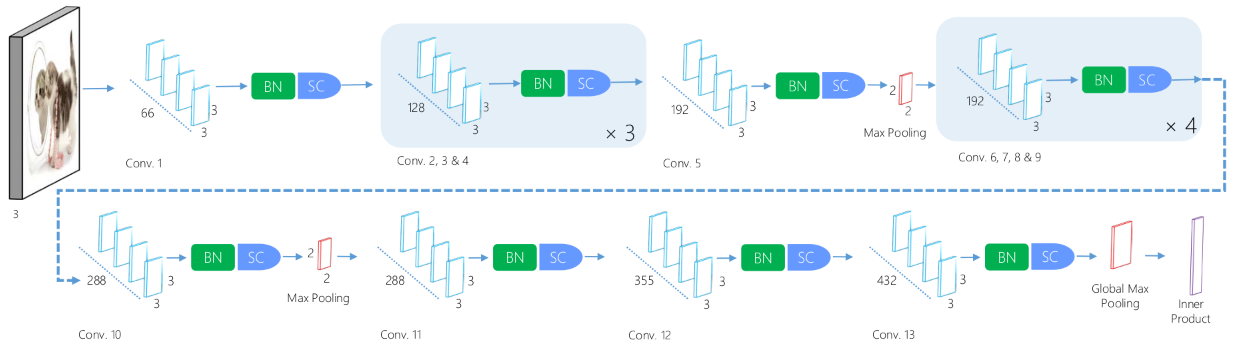
\includegraphics[width=\linewidth]{simpnet-arch.png}
	\caption{\textbf{SimpNet architecture.} Taken from reference article.}
	\label{fig:simpet-arch}
\end{figure*}

\subsection*{Architecture}

For the CNN architecture we have chosen SimpNet \cite{simpnet}, due to its claims to simplicity over other architectures with similar performance in the field of image classification. It consist of 13 convolutional layers with scaling and normalization, 3 max pool layers and 1 fully-connected layer.

Reference implementation of the network was written in Tensorflow, but we have adapted it to Pytorch. This may not have been a good decision since the adaptation may contain mistakes which may have had an impact on overall performance.

When testing the implementation, we have disabled scaling layers and finishing softmax function used in reference implementation due to significantly worse training results. This may be caused by Pytorch already applying these operations "under the hood" or by incorrect configuration of our optimizer and learning parameters.

\subsection*{Dataset}

For this project we have composed an dataset of images obtained by two monitoring studies. The dataset is relatively small and contains two taxonomical orders of species (toad and newts). Some images in the dataset are labeled by individual's name and taxonomical order.

\begin{table}[hbt]
	\caption{Amphibian dataset.}
	\centering
	\begin{tabular}{l | r r r}
		\toprule
		                  & Newts  & Toads    & Total \\
		\midrule
		Images            &        &          & 1722  \\
		Labeled by name   & 293    & 131      & 424   \\
		Names (classes)   & 155    & 30       & 185   \\
		\bottomrule
	\end{tabular}
	\label{tab:amphibian-dataset}
\end{table}

The small dataset causes many problems, one of which is the fact that we cannot use random sampling for splitting the dataset. This is because low number of cases (images) per class cause high probability that some class will not appear in the train subset at all. Is such case, when evaluating the test subset, the network will see some cases for the first time so it will have to guess the corresponding class, which obviously reduces test subset accuracy, but does not mean that the network has not learned feature extraction.

Instead of random sampling, we had split the dataset by hand and filled test subset only with classes that have enough cases so that each subset contains at least two. In this manner, the test subset does not contain classes that do not appear in train subset, but train subset has classes that do not appear in test.

Another problem caused partially by small dataset is overfitting. First measure to overcome it, is data augmentation on the train subset in the form of color jitter and affine transforms. Instead of exploding the dataset into multiple copies with random transformations, Pytorch handles augmentation on per-epoch basis, meaning that the dataset is never copied, but has applied different transformations on every time the images are loaded. This way, the same effect is achieved without data duplication. The transformations and their parameters were chosen based on expected variability of the input images of the same individual over different captures and results during learning phase of classification.

\begin{table}[h]
	\caption{Data augmentation.}
	\centering
	\begin{tabular}{l | r }
		\toprule
		                   & Interval     \\
		\midrule
		Brightness scaling & (0.4, 1.7)   \\
		Contrast scaling   & 20\%         \\
		Saturation scaling & 40\%         \\
		Hue rotation       & 4\%          \\
		Rotation           & $\pm20\deg$  \\
		Translation        & $\pm10\%$    \\
		Scaling            & $\pm10\%$    \\
		Sheer              & $\pm5\%$     \\
		\bottomrule
	\end{tabular}
	\label{tab:augmentation}
\end{table}

\begin{figure}[h]\centering
	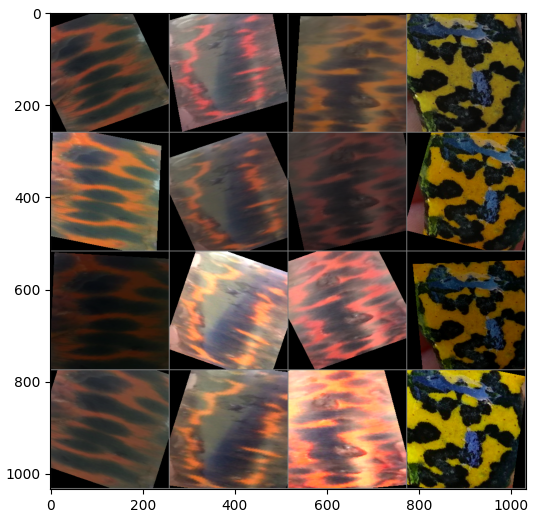
\includegraphics[width=0.8\linewidth]{augmentation.png}
	\caption{\textbf{Dataset augmentation} Each row contains cases loaded for one epoch, each column contains one individual.}
	\label{fig:augmentation}
\end{figure}

To make the problem with small dataset even worse we also need a subset of images to test identification. Individuals in this subset must not appear in train subset, to reflect the open dataset problem we are trying to solve. We handpicked classes with exactly two images, with intention not to disturb classes with many images, which we suspect are most useful in the learning phase. We have named the new subset \textit{ident}.

\newpage
Due to uncertainty of the many decisions regarding the dataset we have experimented and trained 4 different DNN:
\begin{description}
	\item[Net 1] Only \textit{train} and \textit{test} subsets. Goal is to set benchmark for other networks. Cannot be objectivity used to evaluate identification.
	\item[Net 2] \textit{Train}, \textit{test} and \textit{ident} subsets. First try at identification. 
	\item[Net 3] Removed all classes with only one case. This reduced number of images by 67, but brought number of images per class from $2.3$ to $3.1$. Because all images were in train subset, we have moved some images from test and indent to the train subset.
	\item[Net 4] Moved all images from test to train subset. This greatly increased difficulty during classification training as we had no good indication of current accuracy, but ensured that there was more images in the training subset.
\end{description}


\begin{table}[h]
	\caption{Dataset experimentation.}
	\centering
	\begin{tabular}{l r r r r}
		\toprule
		          & Classes & Train       & Test       & Ident      \\
		\midrule
		Net 1     & 185     & 307; 71\%   & 75; 17\%   & 126; 29\% \\
		Net 2     & 185     & 272; 63\%   & 75; 17\%   & 86; 20\% \\
		Net 3     & 118     & 230; 63\%   & 66; 18\%   & 70; 20\% \\
		Net 4     & 185     & 363; 84\%   & 0; 0\%     & 70; 16\% \\
		\bottomrule
	\end{tabular}
	\label{tab:dataset-experimentation}
\end{table}

\subsection*{Detection}

Detection is an important part of the identification pipeline and its implementation is more straight forward than the feature extraction. This is why we have chosen to replace automatic detection with manual labeling of the belly regions.

Also, manual labeling increases amount of work to perform on $n$ images by the order of $O(n)$, which means that the speedup for large datasets from automatization of detection is much lesser than automatic matching. 

\begin{figure}[!h]\centering
	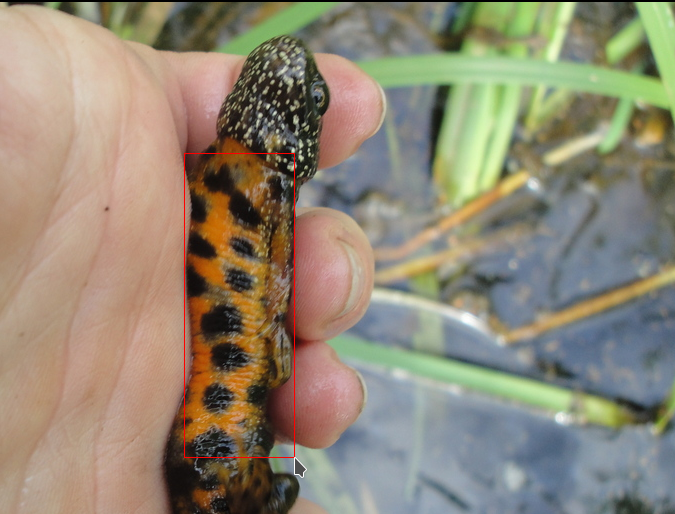
\includegraphics[width=0.8\linewidth]{labelling.png}
	\caption{\textbf{Manual labelling (detection).} We have used Python scripts and OpenCV annotate tool. Input images are expected to be in vertical orientation, labeled pattern should include only the belly pattern. }
	\label{fig:manual-labelling}
\end{figure}

\subsection*{Classification learning}

There are also advantages to the small dataset, prominent of which is more \textit{interactive} learning. Since the number of images to process in one epoch is small, we can observe learning progress in realtime and make adjustments around every 60 epochs which took around 2 minutes on our setup.

First we have tried to train the classifier to only distinguish between the two taxonomical orders of the amphibians, which succeeded very quickly, and then transitioned to distinguishing between individuals. Now the network had quickly started overfitting and reached \>95\% accuracy on the training subset in less than 20 epochs while test accuracy remained under 10\%. 

As described before, the first technique employed to prevent overfitting was dataset augmentation. Over training multiple networks, we have found that the most efficient way of training is to start with no augmentation, letting the model overfit, then enabling light augmentation (approximately half the interval described in table \ref{tab:augmentation}) and at last heavy augmentation that can be seen in figure \ref{fig:augmentation}.

\begin{figure*}[ht]\centering
	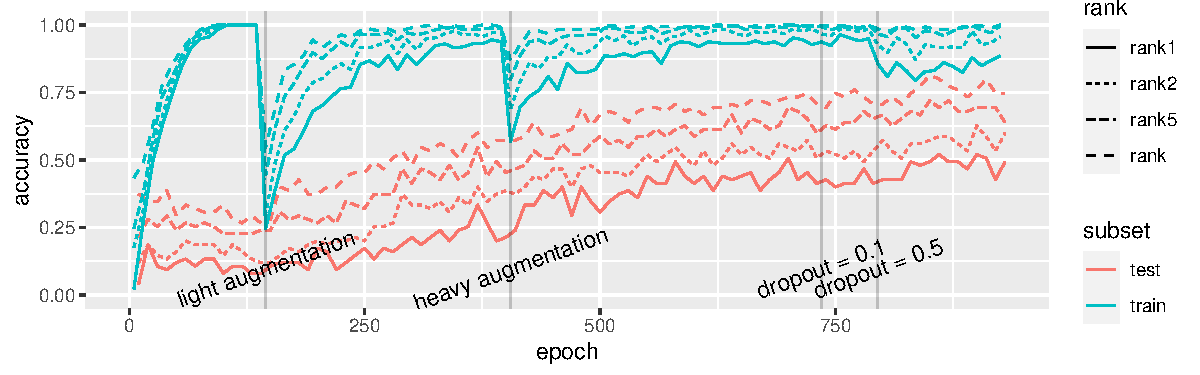
\includegraphics[width=\linewidth]{learning-progress-ranks.pdf}
	\caption{\textbf{Learning progress of net 2} In this case, we can see that after enabling augmentation, the accuracy on train subset drops, but then steadily rises together with test accuracy. Dropout has similar effect but in this case, much lesser.}
	\label{fig:learning-progress}
\end{figure*}

To prevent overfitting even further, we have used dropout; setting random layer outputs to zero and thus preventing the network to use same "activation paths" for classification of a specific image. Each output is zeroed with probability $p$. We have found that applying dropout is most effective after and in combination with heavy augmentation. The most effective learning runs were observed with parameters $p = 0.5$.

We have also found that enabling heavy augmentation and dropout with $p = 0.5$ at the first 100 epochs of model training resulted in sudden drop in accuracy on train and test subsets.

With most efficient combination of overfitting prevention, our models finished learning after just 600 epochs (approximately 20 minutes).

\begin{table}[hbt]
	\caption{Classification accuracy at different ranks.}
	\centering
	\begin{tabular}{l r r r r}
		\toprule
		rank & net1     & net2     & net3    \\
		\midrule
		R1   & 60.3\%  & 54.7\%  & 50.0\% \\
		R2   & 67.5\%  & 58.7\%  & 56.0\% \\
		R3   & 69.0\%  & 65.3\%  & 63.6\% \\
		R5   & 74.6\%  & 72.0\%  & 68.1\% \\
		R10  & 82.5\%  & 78.7\%  & 77.3\% \\
		\bottomrule
	\end{tabular}
	\label{tab:classification-results}
\end{table}

\begin{figure}[htb]\centering
	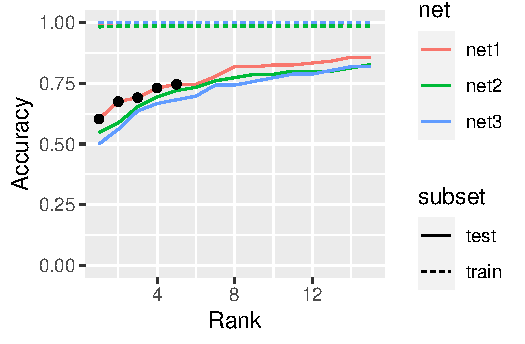
\includegraphics[width=0.9\linewidth]{ranks-classification.pdf}
	\caption{\textbf{Classification (closed dataset) results.} Net 4 is not shown due to empty test subset.}
	\label{fig:classification-results}
\end{figure}

\newpage
\subsection*{Feature extraction}

As we described, our intention is to remove the last or last few layers of the network and obtain outputs of previous layers to be used as a feature vector. But chosen architecture of our network is not very convenient for such procedures, since it has only one fully connected layer, which maps from previous convolutional layer to the output of the network (i.e. activation of our classes). If we were to take output of convolutional layer, feature vector would contain $110.592$ entries, which is much more that expected for a feature vector.

\newpage

We had three options:
\begin{enumerate}
	\itemsep0em
	\item Use output of convolutional layer 13 ($110.592$ outputs)
	\item Use output of convolutional layer 11 ($73.728$ outputs)
	\item Replace fully connected layer with two fully connected layers: first one (fc1) maps from $110.592$ outputs to 256 and the second one (fc2) maps from 256 outputs of (fc1) to our classes. Now retrain the only last two layers and use the output of fc1 as feature vector of more appropriate size.
\end{enumerate}

As all approaches are uncertain, we have explored each of them and compared results in figure \ref{fig:ranks-layer-selection}.

\begin{figure}[htb]\centering
	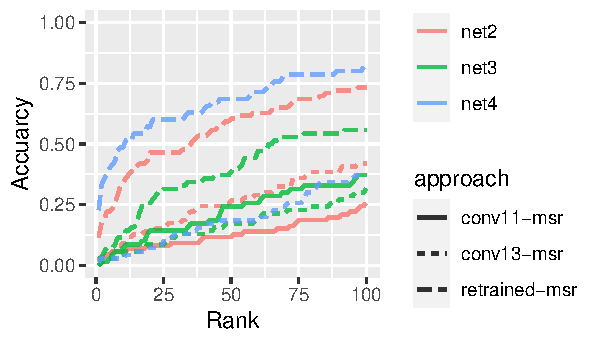
\includegraphics[width=\linewidth]{ranks-ident-layer-selection.pdf}
	\caption{\textbf{Layers used for feature extraction.} We can clearly see that retraining approach achieves best results on all three networks trained.}
	\label{fig:ranks-layer-selection}
\end{figure}

For matching of the feature vectors we have also experimented with Mean Squared Residuals and Cosine similarity as distance measures. We have observed insignificant differences in their performance.

%------------------------------------------------

\newpage
\section*{Results}

From the table \ref{tab:classification-results} we can see that classification accuracy of R1 is around 60\%. After feature extraction, the accuracy drops to 22\% as seen in table \ref{tab:identification-results}. Accuracy of identification at rank 10 is 48\%.

\begin{table}[hbt]
	\caption{Identification accuracy at different ranks.}
	\centering
	\begin{tabular}{l r r r}
		\toprule
		rank & net2    & net3    & net4   \\
		\midrule
		R1   & 11.6\%  &  2.9\%  & 22.9\% \\
		R2   & 17.4\%  &  2.9\%  & 32.9\% \\
		R3   & 18.6\%  &  5.7\%  & 35.7\% \\
		R4   & 22.1\%  &  7.1\%  & 37.1\% \\
		R5   & 22.1\%  &  7.1\%  & 40.0\% \\
		R10  & 33.7\%  & 11.4\%  & 48.6\% \\
		R100 & 73.2\%  & 55.7\%  & 82.9\% \\
		\bottomrule
	\end{tabular}
	\label{tab:identification-results}
\end{table}

\begin{figure}[htb]\centering
	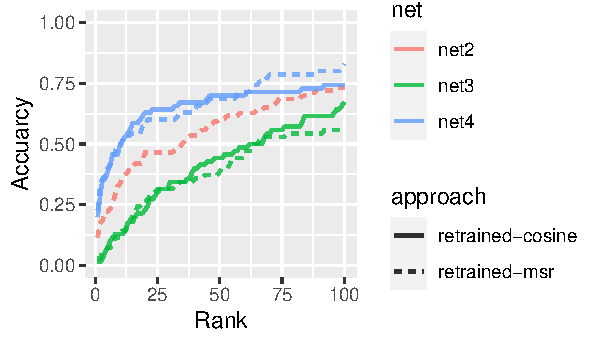
\includegraphics[width=\linewidth]{ranks-ident-nets.pdf}
	\caption{\textbf{Accuracy over ranks after feature vector matching.} (Results of identification on an open dataset) As expected Net 4 performed best, but overall results are not good enough for practical use. Removing classes with single image (net 2) significantly decreased identification accuracy.}
	\label{fig:ranks-ident-nets}
\end{figure}

\section*{Discussion}

Given small dataset, the classification results are relatively good. Having experience with manual matching ourselves, we weren't expecting such high accuracy given small dataset. This is because when performing manual matching, we have more information about where to look for matches. For example, we know that none of the images from same capture belong to the same individual. When evaluating classification and identification, we have instead used worst case scenario and discarded all such heuristic information.

Additionally, the problem has unconstrained environment with high variation of poses and lightning of the individuals, which sometimes greatly increases difficulty even for performing manual matching.

Nevertheless, we weren't expecting such drop in accuracy when transitioning to open dataset (classification vs identification). For net 2 the rank 1 accuracy drops for almost factor 5. This may be solved by employing better distance measures or advanced decision making such as SVM or another neural network.

In our opinion, the most important factor to improve the results would be to extend the dataset. During the research we have extended the dataset with 93 new images which increased classification accuracy by 20\% (this may also be attributed to different augmentation or dropout parameters). From the figure \ref{fig:ranks-ident-nets} we can also see the impact of larger train subset. 

New images could be obtained from local monitoring studies or from authors of referenced articles which compared pattern matching systems \cite{ident_comparison}. Obtaining the dataset used in this comparison study would also allow us to compare the results with similar systems which would be a good indication whether or not this is a feasible approach to the problem. Currently, the achieved metrics are not comparable, since out approach works with much less constrained environments than the referenced study.

Another approach to improve the results would be to replace the architecture of the neural network or to use a pre-trained model as a training starting point. Choosing carefully, we could eliminate the need to replace and retrain last fully connected layer, which may in its own increase identification performance.

\section*{Appendix}

All of the code, statistics and trained models are accessible at Github: \url{https://github.com/aljazerzen/data-science-amph-ident}.

%----------------------------------------------------------------------------------------
%	REFERENCE LIST
%----------------------------------------------------------------------------------------
\bibliographystyle{unsrt}
\bibliography{report}

\end{document}
